\chapter{Design \& Implementation}

After thoroughly researching both how fingerprinting works and how best to mitigate it, the design of the main application began.
The application that was designed and implemented is a browser add-on using the WebExtension API\@.
This is a browser add-on system that is cross-platform, compatible with Firefox, Chrome and Opera, though only Firefox was targeted due to scope and the limited timeframe available for the project.
WebExtensions have two primary types of script, one is a background script which runs across all tabs, the second is a content scrip, which is run in each tab individually.
I decided to use a combination of Firefox settings and preferences and the add-on itself to mitigate fingerprinting, as some of the settings themselves were vital to disabling fingerprinting.
The project originally aimed to do several things, outlined below.

\subsection{Alter Passive Properties}

This first feature of the application was to spoof passively transmitted properties in HTTP requests, such as User Agent.
After studying the WebExtension API, I found the \texttt{webRequest} object \citep{webRequest}.
This can have an \texttt{eventListener} attached to it to wait for a certain event to trigger, and once this event triggers, the add-on can execute code before the browser continues with the request.
Included in these events is the \texttt{onBeforeSendHeaders} event, which is what I originally used.
The full flow of a HTTP request in the browser is displayed in Figure~\ref{fig:webRequest-flow}.

\begin{figure}[h]
\caption{Showing the event flow for a HTTP request}
\fbox{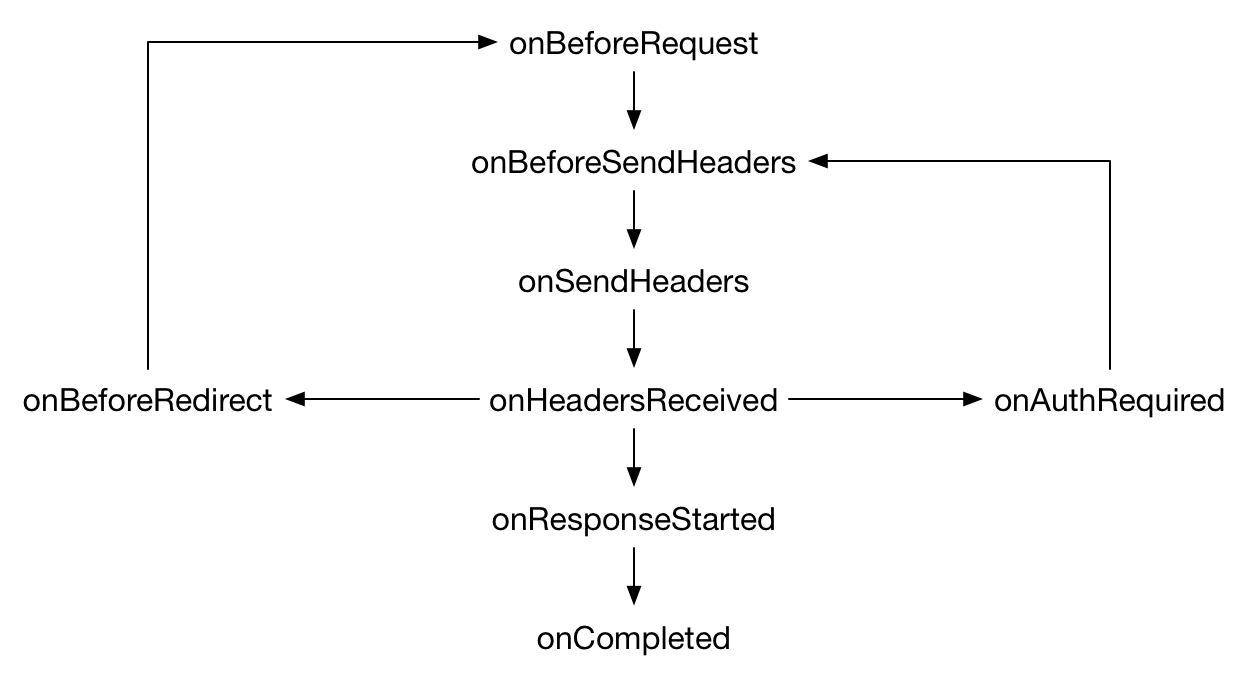
\includegraphics[scale=0.22]{webRequest-flow}}
\centering
\label{fig:webRequest-flow}
\end{figure}

The add-on in this case acts as a proxy between the browser and the website, changing the traffic before passing it on.
Listing~\ref{lst:user-agent} shows background script at an early stage of development that alters the User Agent to a pre-defined one (using Windows and Chrome).
Using this same method, I was able to change other headers, such as editing the date header to have a different timezone than the actual timezone of the computer or changing the HTTP\_ACCEPT headers.

\begin{lstlisting}[caption={The callback used to change the User Agent header}, label={lst:user-agent}]
var ua = "Mozilla/5.0 (Windows NT 10.0; Win64; x64) AppleWebKit/537.36 (KHTML, like Gecko) Chrome/55.0.2883.87 Safari/537.36";

function headerCallback(requestDetails) {
    for (var header of requestDetails.requestHeaders) {
        if (header.name.toLowerCase() === "user-agent") {
                        header.value = ua;
                                
        }
            
    }
        return {requestHeaders: requestDetails.requestHeaders};

}

browser.webRequest.onBeforeSendHeaders.addListener(headerCallback, {urls: ["<all_urls>"]}, ["requestHeaders", "blocking"]);
\end{lstlisting}

After doing more research, I came to realise that spoofing the User Agent for a more common user agent is only going to work against the computer against anything more than the simplest of fingerprinters.
This is because of the different functionality of different browsers can be queried and by process of elimination, the browser and version quickly identified.
By spoofing the value, it makes it more obvious to a complex fingerprinter what the user's identity is, as so few browsers spoof this information.
For this reason, the final iteration of the add-on does not alter the User Agent header.
In addition to this, the timezone header is not altered because of problems with usability for sites that depend on accurate timing information.
These are some of the first problems I ran into, but it was neither the last time I had to ask myself ~`Is concealing or spoofing this characteristic doing more harm than good?' nor was it the last time I had to consider the balance of usability and privacy.

\subsection{Flash Prevention}

Removing or at the very least limiting Flash usage was a key part of the project, since it reveals so much information to fingerprinters.
Luckily Firefox and other commonly used browsers supply preferences for disabling Flash, on Firefox users can disable it altogether or change it to a `click-to-play' setting, where if a page uses Flash an alert will appear asking the user if they'd like to grant the site permission to use Flash once, forever, or to ignore the request.
I considered developing these options into the add-on itself but felt it was redundant with the option already implemented at the browser level.

Due to roughly 10\% of websites using Flash, the `click-to-play' setting is my recommended one to users of the add-on \citep{flash-usage}.
This protect the user against fingerprinters using Flash unless they choose to allow Flash on a specific website.
It unfortunately leaves the decision to the user, and can be difficult to tell why a website would require Flash (eg.\ for watching a video).
With the decline in use of Flash (illustrated in Figure~\ref{fig:flash-usage}) soon the best option will certainly be to disable it altogether, but right now it's difficult to advise to block it altogether when it can cause breakages for many popular websites.

\begin{figure}[h!]
\caption{The decline in Flash usage across the web}
\fbox{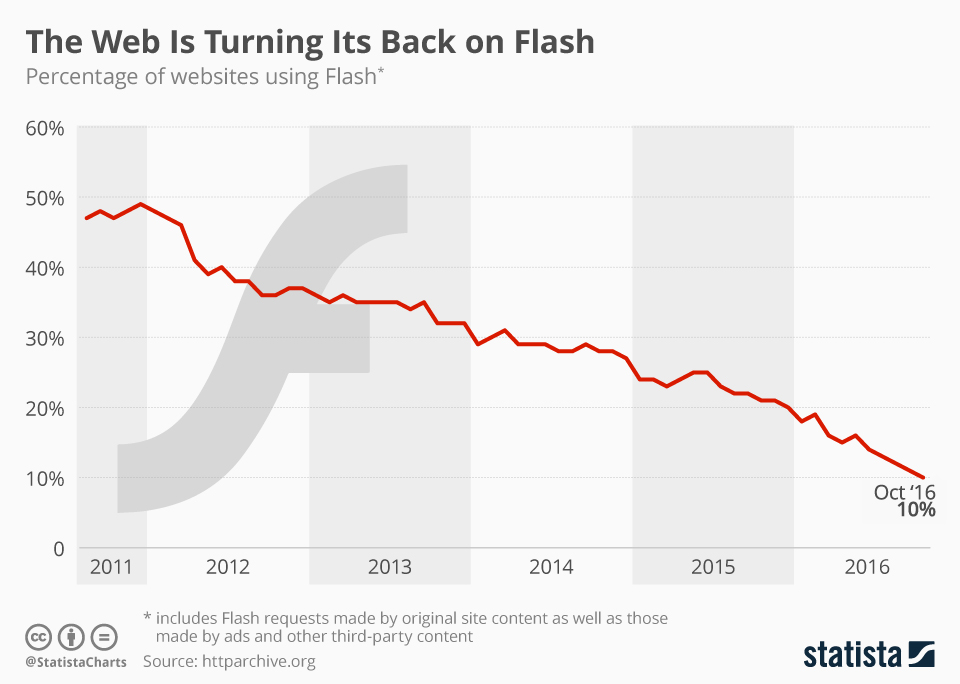
\includegraphics[scale=0.35]{flash-usage}}
\centering
\label{fig:flash-usage}
\end{figure}

\subsection{Font Fingerprinting}

Prevention of font fingerprinting was another important part of the project.
Font fingerprinting through Flash had already been prevented through disabling it altogether, which left the problem of how to stop font fingerprinting through JavaScript.
This was what seemed like an impossible problem, as the browser will use whatever fonts are installed, from extensive research, I could find no method of disabling fonts or concealing them at the add-on level, since it could be altered using CSS, which is too low-level for an add-on to interfere with.

This was a big problem for the project, as font fingerprinting amounts for roughly 7.6 bits of entropy for a sample size of 1,000 users \citep{font-metrics}.
Observing Figure~\ref{fig:font-metrics}, one can see the highest (black) line indicates the maximum entropy if every browser has a unique set of fonts, and the (red) line beneath indicates the entropy available from checking the installed fonts.

\begin{figure}[h!]
\caption{Graph of entropy vs.\ sample size for font fingerprinting.}
\fbox{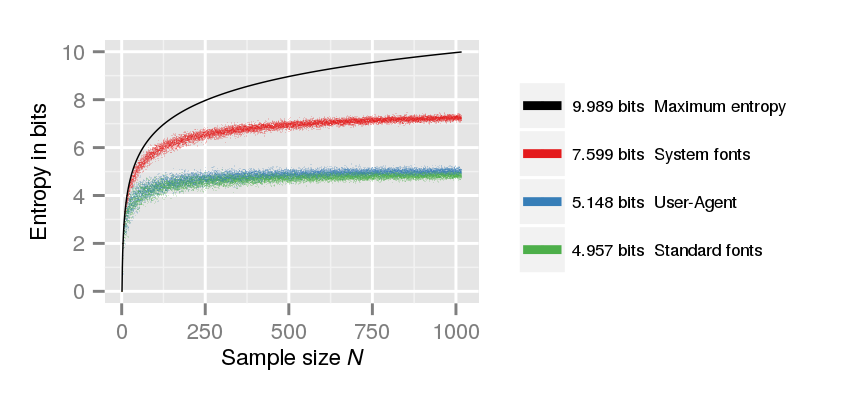
\includegraphics[scale=1.3]{font-metrics}}
\centering
\label{fig:font-metrics}
\end{figure}

Thankfully version 52 of Firefox released on the 7th of March 2017.
In this version of Firefox, a new feature was added that allows users to define a list of `whitelisted' fonts which Firefox will use as if they are the only fonts installed on the system.
This allowed me to change a setting in Firefox's config files, effectively limiting the system fonts to a select few.

\subsection{Prevent Canvas and Audio Fingerprinting}

Preventing Canvas fingerprinting was the most difficult part of the project by far.
This is due to a number of problems and roadblocks I ran into during the development.
The original plan was for the add-on to simply listen to the webpage for changes once it begins to load, and when the page changes, scan any added nodes for any \texttt{<canvas>} elements, and change the objects themselves to restrict the relevant APIs.
This is essentially what the final product does, though it's not as simple as initially thought.

The main methods that need to be blocked are explained in Table~\ref{tab:canvas-methods}.

\begin{table}[h]
\centering
\begin{tabular}{| p{6cm} | p{8cm} |}
    \hline
    \textbf{<canvas> function} & \textbf{Description} \\ \hline
    \texttt{context.measureText()} & {Returns the size of text in the canvas element} \\ \hline
    \texttt{context.getImageData()} & {Returns an object containing data about \newline the canvas element inluding a full pixel map} \\ \hline
    \texttt{canvas.toDataUrl()} & {Returns a URL which contains the canvas \newline itself (fully rendered)} \\
    \hline
\end{tabular}
\caption{Table explaining \texttt{<canvas>} functions that need to be restricted}
\label{tab:canvas-methods}
\end{table}




